\section{Holographie}
A photograph records $|A|^2$ and throws the phase away with it.
\textbf{Holographie} (\textit{holography}), found by D. Gabor in 1948, is the
trick that codes the phase of the onde objet into an intensity pattern a
détecteur quadratique can record, and decodes it again by diffraction. What the
eye receives on read-back is the onde the object itself emitted, so the replica
is genuinely three-dimensional: move in front of the plate and the viewing angle
changes.

\subsection{Importance de la phase et de deux yeux pour la vision en 3D}
D'un point de vue humain, nous avons besoin de deux yeux pour voir en volume.
Les deux yeux voient deux angles de vue légèrement différents et le cerveau
reconstitue la vision volumique.

\begin{definition}[Stéréoscopie]
  Principe de la vision volumique de l'être humain : la \textbf{stéréoscopie}
  (\textit{stereoscopy}). Un observateur regardant une scène voit deux images
  similaires mais légèrement décalées de cette scène avec son œil droit et son
  œil gauche ; le cerveau reconstitue 2 images en 2D décalées en une image 3D.
\end{definition}

D'un autre côté, un objet est rendu visible par les ondes lumineuses qu'il émet,
qu'il réfléchit ou qu'il diffuse. Dans le noir un objet est invisible ! Un objet
quelconque peut être considéré comme constitué d'un ensemble de sources
ponctuelles (principe de Huygens-Fresnel), chacune d'entre elles étant
caractérisée par son spectre dont chaque composante a une \textbf{amplitude} et
une \textbf{phase} déterminée, fonction respectivement de la brillance et de la
position relative du point considéré. C'est la raison pour laquelle un objet
éclairé par une lumière peut être observé de différents endroits : chaque point
de l'objet réémet de la lumière dans toutes les directions.\\

Les informations correspondant à l'amplitude et à la phase sont toutes deux
nécessaires à la perception de l'objet et de son relief. Par exemple, dans le
cas d'une onde plane avec une incidence oblique dans le plan $z=0$, s'exprimant
comme :
\[
  A_0(x,y) = a_0(x,y)\,e^{j\varphi_0(x,y)} = a_0(x,y)\,e^{-jkx\sin\theta}.
\]
Si la phase n'est pas enregistrée, on perd l'information sur la direction
$\theta$ de l'onde --- the factor $e^{-jkx\sin\theta}$ is exactly what
disappears.

\begin{remark}
  L'œil, la pellicule argentique (cristaux d'halogénure d'argent --- AgBr, etc.\
  --- qui noircissent sous l'effet de la lumière ; on obtient un négatif qu'il
  faut développer), le capteur CCD ou CMOS : tous ces détecteurs sont
  \textbf{quadratiques}. All of them respond to $|A|^2$ only. Aucun détecteur ne
  peut enregistrer « l'histoire » de l'onde, i.e.\ its phase.
\end{remark}

\begin{conclusion}
  Amplitude \emph{et} phase doivent être enregistrées si l'on désire restituer
  ultérieurement une réplique fidèle de l'objet en trois dimensions et notamment
  si on souhaite rendre compte de tous les angles de vue, condition nécessaire
  pour que chaque œil voie une vue différente de l'autre. Pour résumer, il faut
  trouver un moyen d'enregistrer \emph{tous les angles de vue sur le même
  support} pour que l'on puisse voir d'une part en volume et d'autre part que la
  vue change lorsque l'on se déplace.
\end{conclusion}

\begin{remark}[3D at the cinema]
  La stéréoscopie au cinéma : les anaglyphes, les images polarisées, les images
  alternées (persistance rétinienne). Écrans 3D sans lunettes, ou
  autostéréoscopie : écrans lenticulaires, écrans lenticulaires multivues,
  écrans parallaxes. All of these exploit stéréoscopie and not holographie, and
  they share the same défauts : besoin de lunettes ou position précise devant
  l'écran ; un seul angle de vue ; focalisation sur l'écran alors que l'objet
  est ailleurs --- mal de tête !
\end{remark}

\subsection{Idée de base de l'Holographie}
En photographie classique, il y a deux raisons pour lesquelles on ne voit pas en
3D.

\begin{subpart}
  \item La première est que lors de la formation d'une image avec une lentille,
    chaque point de l'objet n'éclaire qu'un point de l'image. Un seul angle de
    vue est enregistré. On a beau regarder cette image avec les deux yeux, c'est
    comme si elle avait été enregistrée avec un seul. La vision est en 2D : perte
    des angles de vue, perte de profondeur.
  \item Quand bien même on supprimerait la lentille, la phase n'est pas prise en
    compte : l'image est fixée sur une plaque photographique suivant la
    projection 2D de l'intensité de la lumière que l'objet réfléchit. En effet,
    l'émulsion photographique n'est sensible qu'au module au carré du champ : la
    détection est quadratique. Sans lentille, chaque point de l'objet éclaire
    \emph{l'intégralité} de la plaque ; la plaque est alors (quasi) uniformément
    éclairée, il n'y a pas d'image.
\end{subpart}

\begin{figure}[h!]
  \centering
  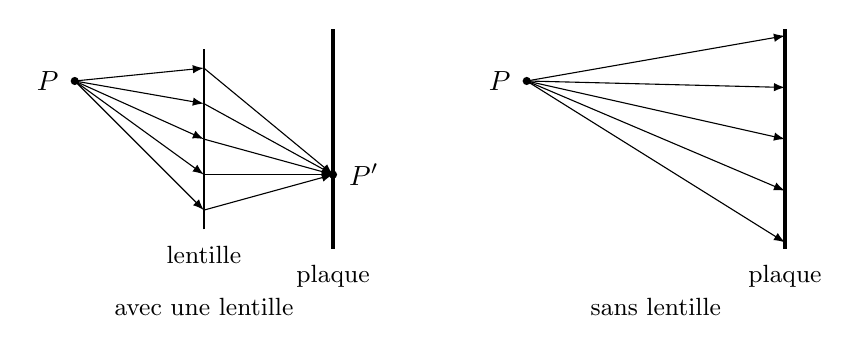
\begin{tikzpicture}[>=latex,scale=0.82]
    % --- with a lens
    \fill (0,0.9) circle (1.8pt); \node[left] at (-0.1,0.9) {$P$};
    \draw[thick] (2,-1.4) -- (2,1.4);
    \node[below] at (2,-1.5) {\small lentille};
    \draw[very thick] (4,-1.7) -- (4,1.7);
    \node[below] at (4,-1.8) {\small plaque};
    \fill (4,-0.55) circle (1.8pt); \node[right] at (4.1,-0.55) {$P'$};
    \foreach \y in {-1.1,-0.55,0,0.55,1.1}{
      \draw[->] (0,0.9) -- (2,\y);
      \draw[->] (2,\y) -- (4,-0.55);
    }
    \node at (2,-2.6) {\small avec une lentille};
    % --- without a lens
    \fill (7,0.9) circle (1.8pt); \node[left] at (6.9,0.9) {$P$};
    \draw[very thick] (11,-1.7) -- (11,1.7);
    \node[below] at (11,-1.8) {\small plaque};
    \foreach \y in {-1.6,-0.8,0,0.8,1.6}{\draw[->] (7,0.9) -- (11,\y);}
    \node at (9,-2.6) {\small sans lentille};
  \end{tikzpicture}
\end{figure}

L'idée de l'holographie est de se donner les moyens d'enregistrer la phase de
l'onde provenant de l'objet. Two conditions follow.

\begin{subpart}
  \item La première condition est de \textbf{supprimer la lentille} pour que
    chaque point de l'objet éclaire l'intégralité de la plaque. Ainsi, chaque
    point de la plaque reçoit l'intégralité de l'information sur l'objet mais vu
    sous un angle donné, c'est-à-dire en 2D. Tous les angles de vue sont
    enregistrés.
  \item La deuxième condition est de trouver un moyen d'enregistrer la phase de
    l'onde objet à l'aide d'un détecteur quadratique puisqu'il n'en existe pas
    d'autres. Pour enregistrer cette phase, \textbf{un code doit être trouvé}
    pour transformer les variations de phase en variations d'intensité.
    L'intensité enregistrée sera ensuite décodée optiquement pour reconstruire
    l'onde initiale. Ce code repose en réalité sur un procédé interférométrique.
    En effet, on sait que si l'on sépare une onde lumineuse en deux faisceaux
    puis qu'on les recombine, l'intensité résultante est une fonction de la
    différence de chemin optique parcouru par les deux ondes (interférences
    constructives ou destructives). C'est un convertisseur de variation de phase
    en variation d'intensité, $\Delta\varphi \to \Delta I$. Il existe donc,
    codée dans la figure d'interférence, une information sur les distances
    relatives des différentes ondes incidentes, donc une information sur le
    volume.
\end{subpart}

\subsection{Éléments de théorie}

\begin{notation}
  The imaginary unit is written $i$ in the general algebra and $j$ in the onde
  plane examples; the two are the same thing. $I_r = |a_r|^2$ et
  $I_0 = |a_0|^2$ sont respectivement les intensités de l'onde de référence et
  de l'onde objet dans le plan $z=0$; $U_0 \equiv A_0$ denotes the onde objet.
  The subscript $r$ is for \textit{référence}, the subscript $0$ for
  \textit{objet}.
\end{notation}

\subsubsection{Enregistrement d'un hologramme}
Le principe du codage holographique est d'enregistrer sur une émulsion
photographique (placée en $z=0$) la figure d'interférences résultant du mélange
entre une onde $A_0$ provenant d'un objet, appelée \textbf{onde objet}
(\textit{object wave}), avec une onde $A_r$ connue, dite \textbf{onde de
référence} (\textit{reference wave}), souvent assimilée à une onde plane. Pour
cela, il faut que les deux ondes soient cohérentes entre elles. L'objet est donc
éclairé par une fraction de l'onde qui sert de référence.

Soit l'expression d'une onde plane choisie comme onde de référence :
\begin{equation*}
  A_r(x,y) = a_r(x,y)\,e^{i\varphi_r(x,y)},
\end{equation*}
avec $|a_r(x,y)|^2$ constant dans le plan de la plaque et $\varphi_r$ dépendant
de l'angle d'incidence :
\begin{equation*}
  \varphi_r(x,y) = \v{k}\cdot\v{r} = k_x x + k_y y + k_z z,
  \qquad \|\v{k}\| = \frac{2\pi}{\lambda},
\end{equation*}
avec $\v{r}$ le vecteur position. Soit l'expression de l'onde objet :
\begin{equation*}
  A_0(x,y) = a_0(x,y)\,e^{i\varphi_0(x,y)},
\end{equation*}
avec $a_0(x,y)$ et $\varphi_0(x,y)$ des expressions compliquées prenant en compte
la somme de l'ensemble des ondes provenant de l'objet. Inutile de détailler ces
deux termes à ce stade. Au point quelconque de coordonnées $(x,y)$, la plaque
reçoit l'amplitude $A_r(x,y)+A_0(x,y)$, et comme l'émulsion photographique n'est
sensible qu'au module au carré du champ,
\begin{equation*}
  I(x,y) \propto |A_r(x,y)+A_0(x,y)|^2
  = |a_r|^2 + |a_0|^2 + a_r^{*}a_0\,e^{-i(\varphi_r-\varphi_0)}
  + a_r a_0^{*}\,e^{i(\varphi_r-\varphi_0)}.
\end{equation*}

\begin{definition}[Hologramme]
  Si la plaque possède, après enregistrement et développement, une transmittance
  $t(x,y)$ \emph{linéairement} proportionnelle à l'intensité enregistrée, alors :
  \begin{equation*}
    \boxed{\;\begin{aligned}
      t(x,y) &\propto |A_r+A_0|^2
      = |a_r|^2+|a_0|^2 + a_r^{*}a_0 e^{-i(\varphi_r-\varphi_0)}
      + a_r a_0^{*}e^{i(\varphi_r-\varphi_0)}\\
      &= I_r + I_0 + 2\sqrt{I_0 I_r}\,
        \cos\!\big[\varphi_r(x,y)-\varphi_0(x,y)\big]
    \end{aligned}\;}
  \end{equation*}
  La transparence obtenue, appelée \textbf{hologramme} (\textit{hologram}),
  contient alors l'information codée sur l'amplitude \emph{et} la phase de $A_0$
  contrairement à une photographie classique --- coded in the cosine term.
\end{definition}

\begin{figure}[h!]
  \centering
  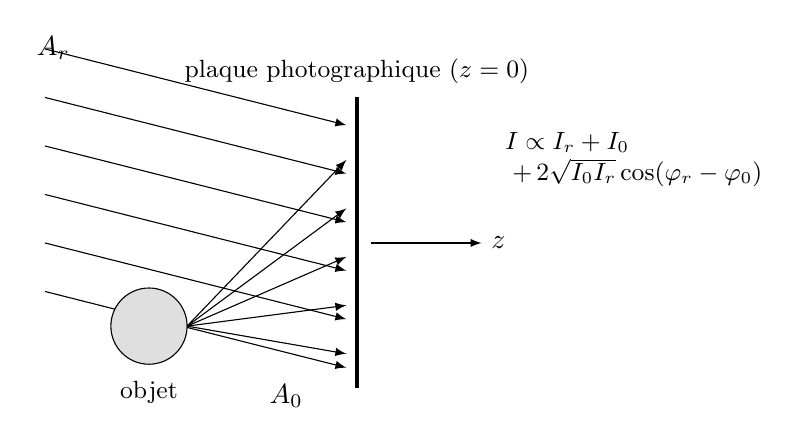
\begin{tikzpicture}[>=latex,scale=0.88]
    \draw[very thick] (3.4,-2.1) -- (3.4,2.1);
    \node[above] at (3.4,2.15) {\small plaque photographique ($z=0$)};
    % reference beam
    \foreach \y in {-1.8,-1.1,-0.4,0.3,1.0,1.7}{\draw[->] (-1.1,\y+1.1) -- (3.25,\y);}
    \node[above left] at (-0.6,2.5) {$A_r$};
    % object
    \draw[fill=gray!25] (0.4,-1.2) circle (0.55);
    \node[below] at (0.4,-1.85) {\small objet};
    \foreach \y in {-1.6,-0.9,-0.2,0.5,1.2}{\draw[->] (0.95,-1.2) -- (3.25,\y);}
    \node[below right] at (2.0,-1.9) {$A_0$};
    \draw[->] (3.6,0) -- (5.2,0) node[right] {$z$};
    \node[right,align=left] at (5.4,1.2)
      {\small $I\propto I_r+I_0$\\[-1pt]\small $\;+\,2\sqrt{I_0I_r}\cos(\varphi_r-\varphi_0)$};
  \end{tikzpicture}
\end{figure}

\subsubsection{Relecture d'un hologramme}
Pour décoder l'information contenue dans l'hologramme et reconstruire l'onde
objet (avec son amplitude et sa phase), l'onde de référence est une nouvelle fois
utilisée pour illuminer l'hologramme. Cette onde va être diffractée par la figure
d'interférence qui est enregistrée sur la plaque. On pourrait étudier en détail
la diffraction de cette onde à distance finie (Fresnel) par l'hologramme mais les
calculs ne sont pas simples. En réalité, il est suffisant d'étudier le champ
transmis \emph{juste après} l'hologramme pour comprendre ce que l'on observe lors
de la relecture. Le résultat est une onde avec une amplitude complexe
$A(x,y) = A_r(x,y)\,t(x,y)$, soit

\begin{theorem}[Les trois ordres de diffraction]
  \begin{align*}
    A(x,y) &= a_r e^{i\varphi_r}\Big[\,|a_r|^2+|a_0|^2
              + a_r^{*}a_0 e^{-i(\varphi_r-\varphi_0)}
              + a_r a_0^{*}e^{i(\varphi_r-\varphi_0)}\Big] \\[2pt]
           &= \underbrace{a_r e^{i\varphi_r}\big(I_r+I_0\big)}_{\text{order }0}
            + \underbrace{|a_r|^2\,U_0}_{\text{order }-1}
            + \underbrace{a_r^2 e^{i2\varphi_r}\,U_0^{*}}_{\text{order }+1}.
  \end{align*}
\end{theorem}

This is the examinable core of the chapter. On distingue dans cette équation
trois termes, appelés \textbf{ordres de diffraction} (\textit{diffraction
orders}), que nous allons détailler --- the three ondes that leave the plate.

\paragraph{Ordre 0 : partie proportionnelle à l'onde de référence.}
\begin{equation*}
  A_{\text{ordre }0} = A_r\,(I_r+I_0).
\end{equation*}
Ce terme représente l'onde de référence modulée par la somme des intensités des
deux ondes initiales. En première approximation, on peut considérer $I_r$ et
$I_0$ uniformes sur la plaque. La direction de $A_{\text{ordre }0}$ est donc
identique à celle de l'onde de référence $A_r$ : il correspond à l'onde de
référence qui traverse l'hologramme sans être diffractée. Il peut être assimilé à
un terme de bruit. En réalité, $I_0$ varie très légèrement sur la plaque suivant
l'objet holographié. Ce terme donne donc lieu à une très faible diffraction de
l'onde plane de référence lors de la reconstruction, que l'on négligera par la
suite ; il peut être appelé « terme ambigu » dans la littérature. Pour négliger
ce terme en pratique, on a coutume également d'augmenter la puissance de l'onde
de référence par rapport à celle de l'onde objet lors de l'écriture.

\paragraph{Ordre $-1$ : partie proportionnelle à l'onde objet.}
\begin{equation*}
  A_{\text{ordre }-1} = |a_r|^2\,U_0 .
\end{equation*}
Ce terme est identique à l'onde objet multipliée par l'intensité de l'onde de
référence. Ce terme reconstitue l'onde objet $A_0$ \emph{en amplitude et en
phase}. On a retrouvé l'objet sous forme d'\textbf{image virtuelle}
(\textit{virtual image}), à l'endroit même où il était lors de l'enregistrement.
L'image restituée est réellement tridimensionnelle : lorsque l'observateur se
déplace devant l'hologramme, l'angle de vue change. On peut décrire l'hologramme
comme une petite fenêtre à travers laquelle on regarderait un objet.

\begin{remark}
  Chaque point de l'objet éclaire l'intégralité de la plaque. Chaque particule
  du matériau photographique contient donc tous les éléments de l'image : elle
  contient l'information de l'ensemble de l'objet mais vu sous un angle donné.
  On peut donc découper un hologramme en plusieurs morceaux et reconstituer avec
  chaque morceau l'image de l'objet entier (en perdant des angles de vue, bien
  sûr).
\end{remark}

\paragraph{Ordre $+1$ : partie proportionnelle à l'onde objet conjuguée.}
\begin{equation*}
  A_{\text{ordre }+1} = a_r^2 e^{i2\varphi_r}\,U_0^{*}.
\end{equation*}
Ce terme, à un facteur d'amplitude près, est l'onde conjuguée de l'onde objet.
C'est une \textbf{image réelle} (\textit{real image}) : elle peut se projeter sur
un écran et même se copier pour dupliquer l'hologramme. Ses profondeurs sont
inversées par rapport à celles de l'objet : l'image réelle est dite
\textbf{pseudoscopique} (\textit{pseudoscopic}) alors que l'image virtuelle est
dite \textbf{orthoscopique} (\textit{orthoscopic}). Le terme de phase
$e^{i2\varphi_r}$ indique la position de l'image réelle ; elle n'est \emph{pas} à
la même position que l'image virtuelle.

\begin{figure}[h!]
  \centering
  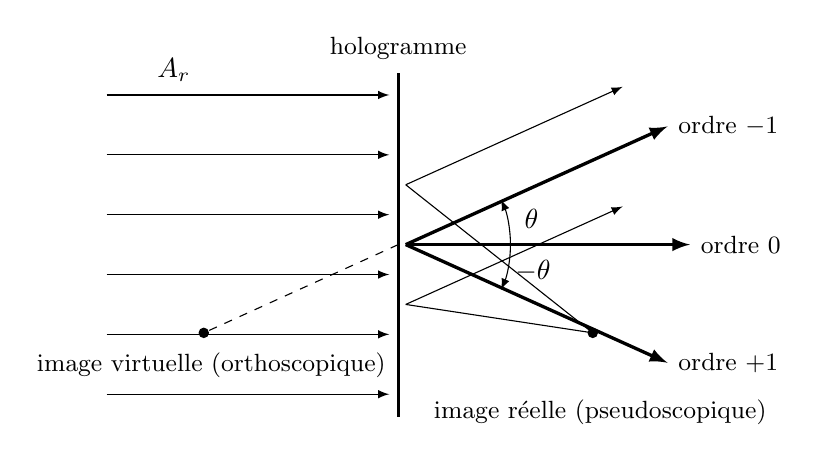
\begin{tikzpicture}[>=latex,scale=0.95]
    \draw[very thick] (0,-2.3) -- (0,2.3);
    \node[above] at (0,2.35) {\small hologramme};
    \foreach \y in {-2.0,-1.2,-0.4,0.4,1.2,2.0}{\draw[->] (-3.9,\y) -- (-0.12,\y);}
    \node[above] at (-3.0,2.05) {$A_r$};
    % order 0
    \draw[->,very thick] (0.1,0) -- (3.9,0) node[right] {\small ordre $0$};
    % order -1
    \draw[->,very thick] (0.1,0) -- (3.6,1.58) node[right] {\small ordre $-1$};
    \draw[->] (0.1,0.8) -- (3.0,2.11);
    \draw[->] (0.1,-0.8) -- (3.0,0.51);
    \draw[dashed] (0,0) -- (-2.6,-1.18);
    \fill (-2.6,-1.18) circle (2pt);
    \node[below] at (-2.5,-1.32) {\small image virtuelle (orthoscopique)};
    % order +1
    \draw[->,very thick] (0.1,0) -- (3.6,-1.58) node[right] {\small ordre $+1$};
    \draw (0.1,0.8) -- (2.6,-1.18);
    \draw (0.1,-0.8) -- (2.6,-1.18);
    \fill (2.6,-1.18) circle (2pt);
    \node[below] at (2.7,-1.95) {\small image réelle (pseudoscopique)};
    \draw[->] (1.5,0) arc (0:23.7:1.5);
    \node at (1.78,0.34) {$\theta$};
    \draw[->] (1.5,0) arc (0:-23.7:1.5);
    \node at (1.80,-0.36) {$-\theta$};
  \end{tikzpicture}
\end{figure}

\begin{remark}[Two sign conventions]
  Two conventions are in use: the ondes written $A = a\,e^{+i\varphi}$, as here,
  or $A(x,y,t) = a\,e^{-i\varphi}e^{i\omega t}$. With the second convention the
  two cross terms swap signs and the three ordres de diffraction read
  $a_r e^{-i\varphi_r}(I_r+I_0) + |a_r|^2 A_0 + a_r^2 e^{-i2\varphi_r}A_0^{*}$.
  The physics is identical; only the sign of every phase exponent changes. Fix
  one convention at the start of a problem and keep it.
\end{remark}

\subsubsection{Hologramme d'une onde plane oblique}
Soit le cas où l'objet est un point lumineux à l'infini. Sur la plaque l'onde
objet est alors une onde plane oblique faisant un angle $\theta$ avec l'axe
$0z$ et une onde de référence plane parallèle à l'axe $0z$
($\varphi_r = 0$). Leur expression peut s'écrire :
\begin{equation*}
  A_r = a_r \qquad\text{and}\qquad A_0 = a_0\,e^{-jkx\sin\theta},
\end{equation*}
où $a_r$ et $a_0$ sont des constantes réelles.

\begin{example}[The three restored waves]
  The general read-back formula gives
  \begin{equation*}
    A(x,y) = \underbrace{a_r\big(I_r+I_0\big)}_{\text{plane wave }\parallel\, 0z}
    \;+\; \underbrace{|a_r|^2 a_0\, e^{-jkx\sin\theta}}_{\text{plane wave at }+\theta}
    \;+\; \underbrace{a_r^2 a_0\, e^{+jkx\sin\theta}}_{\text{plane wave at }-\theta}.
  \end{equation*}
  Le premier terme correspond à une onde plane se propageant dans la direction
  $z$. Le deuxième terme correspond à une onde plane dans la direction $\theta$
  identique à l'onde objet initiale. Le troisième terme correspond à une onde
  plane dans la direction opposée, c'est-à-dire suivant l'angle $-\theta$.
\end{example}

L'onde objet est bien séparée des autres ondes. En fait, cet hologramme est
simplement un enregistrement de franges d'interférences formées par deux ondes
planes se croisant avec un angle $\theta$. Il agit comme un \textbf{réseau de
diffraction sinusoïdal} qui permet de séparer une onde de référence dans trois
directions faisant des angles $0$, $+\theta$ et $-\theta$ par rapport à l'axe
$0z$.

\subsubsection{Hologramme d'un point source à distance finie}
Il est intéressant d'étudier ce cas car tout objet peut être décomposé en une
somme de points sources élémentaires selon le principe de Huygens-Fresnel.
L'hologramme d'un point source peut donc être vu comme l'\textbf{hologramme
élémentaire} (\textit{elementary hologram}). Si l'objet est un point source
situé sur l'axe $0z$ à une distance $-d$ de la plaque holographique, l'onde objet
est une onde sphérique issue du point source dont les coordonnées sont
$\v{r}_0=(0,0,-d)$. L'onde objet peut donc s'exprimer comme :
\begin{equation*}
  A_0(\v{r}) \propto a_0\,\frac{e^{-jk|\v{r}-\v{r}_0|}}{|\v{r}-\v{r}_0|},
  \qquad \v{r}=(x,y,0)\ \text{on the plate}.
\end{equation*}
Une étude détaillée de la figure d'interférence montrerait que l'on obtient une
\textbf{série d'anneaux concentriques}. Term by term:

\begin{subpart}
  \item le premier terme se décompose en une onde plane se propageant dans la
    direction $z$ ainsi qu'un terme proportionnel à $1/|\v{r}-\v{r}_0|^2$ dont
    l'onde se propage dans la direction $z$ avec un angle très petit puisque son
    amplitude varie très lentement dans le plan transverse ;
  \item le deuxième terme est une nouvelle fois similaire à l'onde objet
    initiale : c'est l'\textbf{onde sphérique divergente} qui a été reconstruite.
    Son origine se situe en $(0,0,-d)$, soit exactement la même position que
    celle du point source initial. Cette image est \emph{virtuelle} puisqu'elle
    se forme avant la face de sortie de l'hologramme. Elle ne peut être
    visualisée sur un écran mais peut être imagée par une autre lentille (celle
    de l'œil par exemple) ;
  \item le troisième terme est proportionnel au conjugué de l'onde objet :
    $A_{\text{ordre}+1} \propto a_0\,e^{jk|\v{r}-\v{r}_0|}/|\v{r}-\v{r}_0|$.
    C'est une \textbf{onde sphérique convergente} centrée en $(0,0,+d)$. L'image
    de ce point est donc \emph{réelle} : elle peut être projetée sur un écran.
\end{subpart}

\begin{remark}
  Sur cet exemple, l'onde de référence est parallèle à l'axe $0z$ et le point
  source se trouve sur l'axe. Lors de la restitution, on constate que c'est aussi
  le cas pour l'image conjuguée. On voit qu'il est alors impossible de dissocier
  les différentes images lors de l'observation. Tout est confondu sur l'axe
  $0z$. Note also that the conjugate image of such a hologramme élémentaire
  behaves as a lentille de Fresnel.
\end{remark}

\subsubsection{Holographie hors-axe d'un objet quelconque}
Le moyen de séparer les différentes images est, au moment de l'écriture, de
faire en sorte que l'objet et l'onde de référence ne soient \emph{pas} sur le
même axe optique. On parle alors d'\textbf{holographie hors-axe}
(\textit{off-axis holography}).

Un objet diffusant quelconque peut être considéré comme formé par un grand
nombre de sources ponctuelles d'amplitudes $a_0$ et de phases $\varphi_0$
variables. L'onde diffusée par un objet quelconque peut donc s'exprimer comme :
\begin{equation*}
  f(x,y) = \sum_{\substack{\text{surface}\\ \text{of the object}}} a_0\,e^{j\varphi_0}.
\end{equation*}
Si la direction de cette onde objet fait un angle $\theta$ avec l'axe optique,
c'est une onde dont l'enveloppe complexe $f(x,y)$ portant l'information sur
l'objet est modulée par un facteur de phase qui indique sa direction. The
read-back formula becomes
\begin{equation*}
  A(x,y) \propto a_r e^{i\varphi_r}\Big[I_r + |f(x,y)|^2\Big]
  + |a_r|^2 f(x,y)\,e^{-jkx\sin\theta}
  + a_r^2 f^{*}(x,y)\,e^{+jkx\sin\theta}.
\end{equation*}
Le deuxième terme est une nouvelle fois une réplique de l'onde objet, restituée
avec un angle $\theta$ comme l'indique le terme de phase $e^{-jkx\sin\theta}$.
La présence du facteur $e^{+jkx\sin\theta}$ dans le troisième terme indique que
l'image conjuguée se trouve dans la direction $-\theta$ (par rapport à la
direction de l'onde de référence). Les différentes images restituées sont alors
spatialement séparées et peuvent être observées indépendamment les unes des
autres.

\begin{remark}
  The off-axis onde objet is $A_0(x,y)=f(x,y)e^{-jkx\sin\theta}$, the quantity
  the displayed result uses. Measured from the direction of the onde objet
  rather than from the onde de référence, the conjugate image lies in the
  direction ${\sim}2\theta$ --- the same statement.
\end{remark}

\subsection{Deux familles d'hologrammes : en transmission ou en réflexion}
On a pour habitude d'appeler un hologramme par la manière que l'on utilise pour
le visualiser.

\begin{definition}[Hologrammes en transmission et en réflexion]
  \textbf{Hologramme en transmission} (\textit{transmission hologram}) : on
  regarde le champ transmis par l'hologramme. On place donc lors de la relecture
  son œil de l'autre côté de la plaque --- on the far side from the onde de
  référence.
  \textbf{Hologramme en réflexion} (\textit{reflection hologram}) : on place lors
  de la relecture son œil et l'onde de référence du même côté de la plaque si
  bien que l'on observe les ondes réfléchies par l'hologramme.
\end{definition}

En réalité, ces hologrammes sont très différents. La première différence
concerne la manière dont on enregistre l'hologramme.

\subsubsection{Hologramme en transmission}
Considérons le cas simple où l'onde objet et l'onde de référence sont des ondes
planes cohérentes portées par les vecteurs d'onde $\v{k}_r$ et $\v{k}_0$ à la
longueur d'onde $\lambda_{\text{écriture}}$. Dans le cas d'un hologramme en
transmission, l'objet et l'onde de référence sont placés du \emph{même côté} de
la plaque holographique au moment de l'écriture. L'épaisseur de la gélatine
photographique permettant l'enregistrement s'étend de $z=0$ à $z=\Delta$. Les
franges d'interférences sont alors une fonction des variables $x$, $y$ \emph{et}
$z$ :
\begin{align*}
  I(x,y,z) &\propto \big|a_r e^{-j\v{k}_r\cdot\v{r}} + a_0 e^{-j\v{k}_0\cdot\v{r}}\big|^2\\
           &= I_r+I_0+2\sqrt{I_r I_0}\,\cos\!\big(\v{k}_0\cdot\v{r}-\v{k}_r\cdot\v{r}\big)
            = I_r+I_0+2\sqrt{I_r I_0}\,\cos\!\big(\v{k}_g\cdot\v{r}\big),
\end{align*}
où le vecteur $\v{k}_g = \v{k}_0-\v{k}_r$ est appelé \textbf{vecteur réseau}
(\textit{grating vector}). $I(x,y,z)$ présente des franges d'interférences
sinusoïdales de période $\Lambda = 2\pi/\|\v{k}_g\|$.

Les deux ondes sont cohérentes si bien que
$\|\v{k}_r\|=\|\v{k}_0\|=2\pi/\lambda_{\text{écriture}}$. Les deux vecteurs
faisant un angle $+\theta/2$ et $-\theta/2$ avec l'axe optique, on montre
facilement à l'aide du diagramme des vecteurs que l'expression se simplifie car
$\v{k}_g$ est colinéaire à l'axe $0x$ :
\begin{equation*}
  \v{k}_g\cdot\v{r} = 2\big(\|\v{k}_r\|\sin(\theta/2)\big)x
  = 2\left(\frac{2\pi}{\lambda_{\text{écriture}}}\sin(\theta/2)\right)x,
\end{equation*}
d'où
\begin{equation*}
  I(x,y,z) \propto I_r+I_0+2\sqrt{I_r I_0}\,
  \cos\!\left(2\,\frac{2\pi}{\lambda_{\text{écriture}}}\,x\sin(\theta/2)\right).
\end{equation*}
Les surfaces d'intensité constante (franges d'interférences) sont normales au
vecteur $\v{k}_g$, c'est-à-dire à l'axe $0x$. La période des franges
d'interférence est :
\begin{equation*}
  \boxed{\;\Lambda = \frac{\lambda_{\text{écriture}}}{2\sin(\theta/2)}
  > \frac{\lambda_{\text{écriture}}}{2}.\;}
\end{equation*}
Plus $\theta/2$ augmente, plus $\Lambda$ diminue ; la valeur minimale de
l'interfrange est $\lambda/2$.

\begin{figure}[h!]
  \centering
  \begin{tikzpicture}[>=latex,scale=0.9]
    % --- transmission: emulsion slab, fringes normal to 0x
    \fill[blue!8] (-0.32,-1.5) rectangle (0.32,1.5);
    \draw (-0.32,-1.5) rectangle (0.32,1.5);
    \foreach \y in {-1.2,-0.8,-0.4,0,0.4,0.8,1.2}
      {\draw[red,thick] (-0.32,\y) -- (0.32,\y);}
    \draw[<->] (0.55,0) -- (0.55,0.4); \node[right] at (0.58,0.2) {$\Lambda$};
    \draw[->] (-2.5,1.1) -- (-0.42,0.2); \node[left] at (-2.5,1.1) {$\v{k}_r$};
    \draw[->] (-2.5,-1.1) -- (-0.42,-0.2); \node[left] at (-2.5,-1.1) {$\v{k}_0$};
    \node[align=center] at (-0.7,-2.25)
      {\small en transmission\\[-3pt]\small $\v{k}_g \parallel 0x$, franges $\perp$ surface};
    \draw[->] (-1.5,-3.6) -- (-0.1,-4.05) node[below] {$\v{k}_r$};
    \draw[->] (-1.5,-3.6) -- (-0.1,-3.15) node[above] {$\v{k}_0$};
    \draw[->,very thick] (-0.1,-4.05) -- (-0.1,-3.15);
    \node[right] at (0.0,-3.6) {$\v{k}_g$};
    % --- reflection: fringes parallel to the surface
    \fill[blue!8] (6.08,-1.5) rectangle (6.72,1.5);
    \draw (6.08,-1.5) rectangle (6.72,1.5);
    \foreach \x in {6.16,6.28,6.4,6.52,6.64}
      {\draw[red,thick] (\x,-1.5) -- (\x,1.5);}
    \draw[<->] (6.16,1.72) -- (6.28,1.72); \node[above] at (6.22,1.72) {$\Lambda$};
    \draw[->] (4.1,1.1) -- (5.95,0.35); \node[left] at (4.1,1.1) {$\v{k}_r$};
    \draw[->] (8.7,1.1) -- (6.85,0.35); \node[right] at (8.7,1.1) {$\v{k}_0$};
    \node[align=center] at (6.4,-2.25)
      {\small en réflexion\\[-3pt]\small $\v{k}_g \parallel 0z$, franges $\parallel$ surface};
    \draw[->] (6.4,-3.15) -- (7.6,-3.7) node[right] {$\v{k}_r$};
    \draw[->] (6.4,-3.15) -- (5.2,-3.7) node[left] {$\v{k}_0$};
    \draw[->,very thick] (7.6,-3.7) -- (5.2,-3.7);
    \node[below] at (6.4,-3.78) {$\v{k}_g$};
  \end{tikzpicture}
\end{figure}

Si on enregistre ces franges sur l'émulsion d'épaisseur $\Delta$, ces franges
peuvent être vues comme un réseau de diffraction \emph{épais}. L'hologramme est
appelé \textbf{hologramme de volume} (\textit{volume hologram}). Lorsque ce
réseau est ré-éclairé par une onde plane de longueur d'onde
$\lambda_{\text{relecture}}$ avec le même angle $\theta/2$ que l'onde de
référence initiale, les plans parallèles du réseau de Bragg diffusent la lumière
dans toutes les directions. Dans une direction donnée d'observation $i$, il y a
interférences constructives lorsque la \textbf{condition de Bragg}
(\textit{Bragg condition}) suivante est satisfaite :
\begin{equation*}
  \sin(i) - \sin(\theta/2) = k\,\frac{\lambda_{\text{relecture}}}{\Lambda},
  \qquad k\in\zee .
\end{equation*}

\paragraph{Reconstruction avec une longueur d'onde identique à celle d'écriture.}
Si $\lambda_{\text{relecture}}=\lambda_{\text{écriture}}$, alors, en utilisant
la condition de Bragg et l'expression de $\Lambda$, on montre que :
\begin{equation*}
  \sin(i) = (2k+1)\sin(\theta/2).
\end{equation*}
On constate qu'il existe plusieurs angles (appelés ordres) de diffraction en
fonction de $k$. Pour $k=-1$, $i=\theta/2$ : l'angle de l'ordre $-1$ de
diffraction est égal à l'angle d'incidence de l'onde objet. \emph{L'objet est
reconstitué à la même position que celle initiale de l'objet.} Il existe
d'autres angles où l'on retrouve des répliques de l'objet (other values of
$k$) ; en général, ces répliques sont beaucoup moins intenses.

\paragraph{Reconstruction avec une longueur d'onde différente de celle d'écriture.}
Si $\lambda_{\text{relecture}}\neq\lambda_{\text{écriture}}$, la condition de
Bragg montre cette fois que l'angle de l'ordre $-1$ de diffraction n'est plus
identique à l'angle d'incidence : l'objet ne sera plus au même endroit. On
montre, mais la démonstration n'est pas triviale, que la taille de l'objet est
également modifiée.

\begin{conclusion}
  Un hologramme en transmission sera flou et irisé s'il est éclairé en lumière
  blanche. Un hologramme en transmission doit donc être absolument observé en
  lumière monochromatique. Dans ce cas, si
  $\lambda_{\text{relecture}}\neq\lambda_{\text{écriture}}$, alors la position
  de l'objet restitué change par rapport à sa position initiale mais l'image de
  l'objet reste visible et nette.
\end{conclusion}

\subsubsection{Hologramme en réflexion}
À la différence des hologrammes en transmission, le faisceau de référence et le
faisceau objet sont cette fois placés \emph{de part et d'autre} de la plaque.
L'expression des interférences ne change pas. Par contre, compte tenu des
directions des vecteurs d'onde $\v{k}_r$ et $\v{k}_0$, le vecteur réseau
$\v{k}_g=\v{k}_0-\v{k}_r$ est cette fois parallèle à l'axe $0z$ :
\begin{equation*}
  \v{k}_g\cdot\v{r} = 2\big(\|\v{k}_r\|\cos(\theta/2)\big)z
  = 2\left(\frac{2\pi}{\lambda_{\text{écriture}}}\cos(\theta/2)\right)z,
\end{equation*}
\begin{equation*}
  I(x,y,z) \propto I_r+I_0+2\sqrt{I_r I_0}\,
  \cos\!\left(2\,\frac{2\pi}{\lambda_{\text{écriture}}}\,z\cos(\theta/2)\right).
\end{equation*}
Les franges d'interférences sont \emph{parallèles à la surface} de l'émulsion
photographique (franges dans l'épaisseur). La période des franges d'interférence
devient :
\begin{equation*}
  \boxed{\;\Lambda = \frac{\lambda_{\text{écriture}}}{2\cos(\theta/2)}
  > \frac{\lambda}{2}.\;}
\end{equation*}

Lors de la reconstruction, on ré-illumine l'hologramme avec une onde plane
provenant d'une source blanche et un angle d'incidence $i$ et on regarde le champ
réfléchi par l'hologramme. Son angle de réflexion est identique à l'angle
d'incidence comme nous l'indiquent les lois de Descartes-Snell. Cette onde va
être démultipliée en se réfléchissant sur différents plans d'interférence. On
montre que le déphasage entre une onde réfléchie sous un angle d'incidence $i$
et une autre onde réfléchie qui a traversé une couche supplémentaire est :
\begin{equation*}
  \phi = 2\Lambda\cos(i).
\end{equation*}
On considère qu'une longueur d'onde est réfléchie si le déphasage est un
multiple de $2\pi$. D'après l'expression de l'interfrange $\Lambda$, la longueur
d'onde réfléchie est :
\begin{equation*}
  \boxed{\;\lambda_{\text{réfléchie}}
  = \lambda_{\text{écriture}}\,\frac{\cos(i)}{\cos(\theta/2)}.\;}
\end{equation*}

\begin{conclusion}
  Si l'angle de relecture $i$ est égal à l'angle d'écriture $\theta/2$, la
  longueur d'onde réfléchie sera identique à la longueur d'onde d'écriture. Les
  autres longueurs d'onde ne seront pas réfléchies mais transmises ; ces
  longueurs d'onde ne seront donc pas gênantes. En réflexion, en même temps
  qu'on enregistre un hologramme, on inscrit un filtre appelé \textbf{filtre de
  Bragg} (\textit{Bragg filter}) ou \textbf{miroir de Bragg} (\textit{Bragg
  mirror}) : en réflexion, un hologramme éclairé en lumière blanche sera
  \emph{net et monochrome}. Si au contraire $i \neq \theta/2$, alors
  $\lambda_{\text{réfléchie}} \neq \lambda_{\text{écriture}}$ : lorsqu'on fait
  varier l'angle d'incidence de la lumière blanche, la couleur réfléchie par
  l'hologramme varie mais l'hologramme reste monochrome.
\end{conclusion}

\begin{remark}[Quelques applications des miroirs de Bragg]
  Les miroirs de Bragg sont utilisés dans des domaines de l'optique relativement
  variés comme : traitements antireflets --- lunettes, instruments d'optique
  (télescope, appareil photographique), toutes longueurs d'onde (UV, visible,
  IR) ; lasers --- miroirs haute réflectivité, laser monomode, lasers DFB ou
  VCSEL, affinement de raie laser, lasers à fibre ; fonctions optiques fibrées
  dans les télécommunications --- compensation de dispersion, insertion /
  extraction (Add-Drop) de longueur d'onde dans le réseau. Bien sûr,
  l'empilement des couches peut parfois être très complexe pour obtenir toutes
  sortes de gabarits de filtres.
\end{remark}

\subsection{Contraintes expérimentales}

\subsubsection{Un laser}
Pour enregistrer un hologramme, il faut réaliser des interférences entre une
onde de référence et une onde objet. Cela impose donc de disposer d'une source
cohérente avec un minimum de fluctuations de phase : il faut donc disposer d'un
laser. Le faisceau objet et le faisceau de référence doivent de plus provenir de
la \emph{même} source --- généralement, les deux faisceaux cohérents sont
obtenus en divisant un faisceau laser à l'aide d'une \textbf{lame séparatrice}
(\textit{beam splitter}), par division d'amplitude. On ne peut donc pas
holographier un objet émettant spontanément de la lumière. L'onde objet sera
réalisée par la diffusion d'une onde plane par cet objet, onde cohérente avec
l'onde de référence. La différence de marche entre les deux faisceaux depuis leur
séparation jusqu'à leur recombinaison sur la plaque doit être inférieure à la
longueur de cohérence. Plus la cohérence du laser sera grande, plus le volume des
objets holographiés pourra être grand.

\begin{remark}
  On utilise des lasers à émission continue pour enregistrer des objets
  inanimés. Pour les scènes animées, on utilise des lasers impulsionnels. Une
  impulsion de très forte énergie et d'une durée de l'ordre de la nanoseconde
  permet par exemple de figer une balle à la sortie d'un canon de fusil !
\end{remark}

\subsubsection{Les plaques holographiques}
Une plaque est constituée de grains sensibles à la lumière. Lorsque cette plaque
est plongée dans une solution de révélation, les grains ayant reçu de la lumière
noircissent alors que les autres restent transparents. Three constraints follow.

\paragraph{Taille des grains.}
Puisque les franges d'interférence que l'on souhaite enregistrer sont composées
de fines lignes dont la séparation peut être aussi petite que $\lambda/2$, les
grains de l'émulsion photographique doivent pouvoir discriminer une frange
brillante d'une frange sombre espacées de $\lambda/4$. Leur taille doit donc être
très inférieure à cette valeur. Si le laser d'inscription est un HeNe, la taille
du grain doit alors être très inférieure à $150\,$nm. Les émulsions comportent
donc entre $50\,000$ et $125\,000$ traits/mm (contre
environ $200$ traits/mm pour la photographie classique), soit une taille de grain
qui peut atteindre $8\,$nm contre $5\,\mu$m pour la photographie. En
contrepartie, le film est beaucoup moins sensible et les temps de pose sont de
l'ordre de quelques secondes.

\paragraph{La linéarité de la réponse de la plaque.}
La relation qui nous intéresse est celle qui relie l'amplitude $t$ transmise par
la plaque à l'énergie $W$ reçue par la plaque pendant l'enregistrement. Pour
atteindre la zone de linéarité requise pour enregistrer correctement les franges
d'interférences avec un bon contraste, le temps de pose doit être adapté ---
around the mean received energy $W_0$. En deçà ou au-dessus, le
contraste des franges enregistrées diminue dramatiquement et également en
conséquence l'efficacité de diffraction. L'objet restitué perd en luminosité. Le
choix du temps de pose est donc primordial.

\begin{figure}[h!]
  \centering
  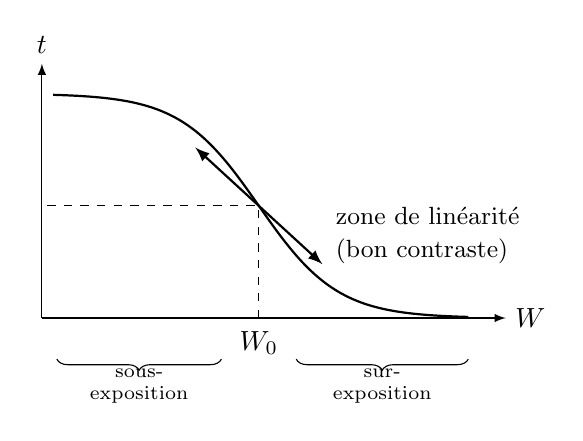
\begin{tikzpicture}[>=latex,scale=0.95]
    \draw[->] (0,0) -- (6.2,0) node[right] {$W$};
    \draw[->] (0,0) -- (0,3.4) node[above] {$t$};
    \draw[thick,domain=0.15:5.7,samples=80,smooth]
      plot (\x,{3/(1+exp(1.9*(\x-2.9)))});
    \draw[dashed] (2.9,0) -- (2.9,1.5) -- (0,1.5);
    \node[below] at (2.9,-0.05) {$W_0$};
    \draw[<->,thick] (2.05,2.28) -- (3.75,0.72);
    \node[right,align=left] at (3.8,1.1) {\small zone de linéarité\\\small (bon contraste)};
    \draw[decorate,decoration={brace,mirror,amplitude=4pt}] (0.2,-0.55) -- (2.4,-0.55)
      node[midway,below,font=\scriptsize,align=center] {sous-\\exposition};
    \draw[decorate,decoration={brace,mirror,amplitude=4pt}] (3.4,-0.55) -- (5.7,-0.55)
      node[midway,below,font=\scriptsize,align=center] {sur-\\exposition};
  \end{tikzpicture}
\end{figure}

\paragraph{Épaisseur des plaques.}
Pour les hologrammes en réflexion, les franges sont parallèles à la surface de
l'hologramme. Pour que le filtre de Bragg soit suffisamment efficace, il faut
enregistrer quelques franges. L'épaisseur de la gélatine doit donc être
supérieure à quelques $\Lambda$, sans quoi il est impossible de réaliser un
hologramme en réflexion. Cette épaisseur n'est pas requise pour les hologrammes
en transmission.

\subsubsection{La stabilité du montage pendant l'inscription}
Puisque l'écart entre une frange brillante et une frange sombre peut être aussi
petit que $\lambda/4$, une vibration peut faire bouger ces franges pendant
l'enregistrement --- la prise de vue peut prendre de quelques secondes à
quelques minutes --- et donc diminuer le contraste des franges enregistrées,
voire les annuler. Il faut donc se donner les moyens de diminuer au maximum les
perturbations extérieures : vibration du montage par le sol, par la ventilation
des appareils, par des bruits acoustiques, vibration de la plaque, mouvement de
l'objet ; variation de température, de pression ou d'hygrométrie ; convection
par le chauffage, par des mouvements dans la pièce, par la chaleur des personnes
ou leur respiration ; gradients thermiques sur la plaque.

\subsubsection{Montage expérimental typique en transmission}
Chaque montage holographique est unique. Il en existe une infinité suivant
l'objet que l'on holographie, l'application, l'angle de vue que l'on souhaite de
l'objet ou de l'onde de référence (qui sera le même en écriture qu'en
relecture). Pour un hologramme en transmission, les règles essentielles à
respecter sont : respect de la cohérence mutuelle des deux ondes ; les deux
ondes doivent être du \emph{même côté} de la plaque. A laser beam is divided on
a lame séparatrice, one arm illuminating the object and the other reaching the
plate directly; at read-back the reference arm alone is restored and the
observer looks through the plate.

\subsubsection{Montage expérimental typique en réflexion : Hologramme de Denisyuk}
Pour un montage en réflexion, les remarques sont les mêmes que pour un
hologramme en transmission si ce n'est que les deux ondes doivent cette fois
arriver \emph{de part et d'autre} de la plaque.

\begin{definition}[Hologramme de Denisyuk]
  L'\textbf{hologramme de Denisyuk} (\textit{Denisyuk hologram}), inventé par
  Y.\,N.\ Denisyuk en 1962, est le montage le plus simple qui soit. C'est un
  hologramme à \emph{faisceau unique} où, au moment de l'écriture, la plaque
  holographique sert elle-même de lame séparatrice. The expanded laser beam
  crosses the plate and plays the part of the onde de référence; the light it
  scatters back off the object, placed just behind the plate, is the onde objet.
\end{definition}

\begin{figure}[h!]
  \centering
  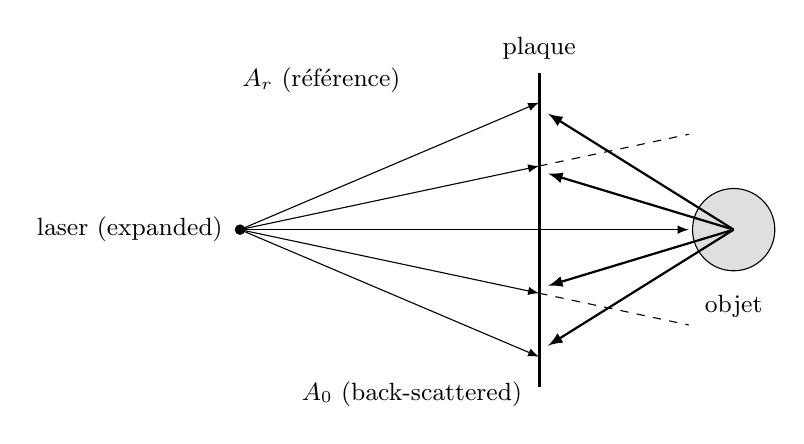
\begin{tikzpicture}[>=latex,scale=0.95]
    \coordinate (S) at (-4.0,0);
    \fill (S) circle (2pt);
    \node[left] at (-4.1,0) {\small laser (expanded)};
    \draw[very thick] (0,-2.1) -- (0,2.1);
    \node[above] at (0,2.15) {\small plaque};
    \foreach \y in {-1.7,-0.85,0.85,1.7}{\draw[->] (S) -- (0,\y);}
    \draw[->] (S) -- (2.0,0);
    \foreach \y in {-0.85,0.85}{\draw[dashed] (0,\y) -- (2.0,{1.5*\y});}
    \draw[fill=gray!25] (2.6,0) circle (0.55);
    \node[below] at (2.6,-0.75) {\small objet};
    \foreach \y in {-1.55,-0.75,0.75,1.55}{\draw[->,thick] (2.6,0) -- (0.12,\y);}
    \node[right] at (-4.1,2.0) {\small $A_r$ (référence)};
    \node[below] at (-1.7,-1.9) {\small $A_0$ (back-scattered)};
  \end{tikzpicture}
\end{figure}

L'hologramme de Denisyuk présente l'avantage d'avoir un réalisme extraordinaire.
Les ombres enregistrées semblent être recréées par la source de référence au
moment de la restitution. Rien de mieux pour tromper l'observateur, même averti !
Il est en plus visible en lumière blanche --- it is a hologramme en réflexion.

\subsection{Applications de l'holographie}
Hormis la réalisation d'images impressionnantes, l'holographie possède
énormément d'applications dans des domaines aussi variés que l'industrie ou la
médecine. L'avènement du numérique dans ce domaine promet un bond en avant
exceptionnel ces prochaines années.

\paragraph{Holographie couleur et muséographie.}
Longtemps inapplicables en muséologie parce qu'ils étaient monochromes et donc
peu réalistes, les hologrammes ont vu leurs domaines d'application s'étendre
depuis la mise au point des hologrammes couleur par Y.\ Gentet, fin des années
90. La difficulté résidait dans l'invention de gélatines sensibles à tout le
spectre visible. Pour rendre compte des couleurs, il suffit alors d'utiliser
trois lasers différents (bleu, vert et rouge) pour enregistrer les hologrammes.
Désormais, dans les musées, certaines œuvres, trop précieuses ou trop fragiles
pour être exposées, sont holographiées avec la plus grande précision. Leurs
images 3D sont alors exposées avec une qualité comparable à l'original.

\paragraph{Photo-inscription et composants optiques.}
Les réseaux de Bragg sont des composants très utilisés dans les réseaux de
télécommunications, notamment dans les commutateurs, les routeurs, les systèmes
de changement ou de décalage spectral. Ils sont utiles pour extraire ou insérer
des longueurs d'onde dans le réseau et compenser la dispersion chromatique. Les
franges de modulation périodique d'indice de réfraction constituant un réseau de
Bragg sont photo-inscrites par laser UV (franges d'interférences UV) dans le
cœur d'une fibre optique monomode (dopage Ge), l'indice du verre étant rendu
dépendant de l'insolation UV qu'il reçoit. Lorsqu'il est ensuite éclairé, ce
réseau se comporte comme un « miroir » pour une bande spectrale très fine autour
d'une longueur d'onde caractéristique (dite « de Bragg »), et transmet toutes les
autres. Dans les technologies DWDM (Dense Wavelength Division Multiplexing), les
informations sont transmises sur une même fibre mais dans des canaux adjacents
caractérisés par des longueurs d'onde différentes. Le réseau de Bragg est un
filtre très sélectif qui ne réfléchit que la longueur d'onde souhaitée. Ainsi,
les multiplexeurs à insertion-extraction peuvent extraire un canal dans le flot
qui arrive à un nœud du réseau puis éventuellement le réinsérer en aval. Les
égalisateurs de gains pour amplificateurs optiques sont également réalisés grâce
à des réseaux de Bragg « longue période » ou « blasés ». Enfin, grâce à des
réseaux à pas variable (dits « chirpés »), on n'a plus seulement une longueur
d'onde concernée par la diffraction mais un continuum de longueurs d'onde, et
cet élargissement du spectre permet d'effectuer de la compensation de
dispersion.

Certains types d'hologrammes agissent sur la lumière mais ne forment pas
d'images 3D : ce sont les \textbf{éléments d'optique holographiques}
(\textit{holographic optical elements}, EOH). Ils consistent à former
l'hologramme d'une optique de base (lentille, lame séparatrice…). L'holographie
permet la création de différents réseaux, dont les densités de traits peuvent
aller de $65$ à plus de $5000$ traits/mm : plans, courbes (concave…), corrigés
des aberrations. Ils sont meilleurs que les réseaux gravés du fait de leur
faible taux d'imperfection. On peut citer la réalisation d'optiques spéciales
pour la focalisation (lentilles holographiques), la séparation ou la déviation
de faisceaux laser, la réalisation de faisceaux pour la spectroscopie, de filtres
d'amplitude et de phase pour la reconnaissance de forme, la correction des
aberrations, l'adressage. Un exemple d'utilisation est la réalisation d'un
tableau de bord composé d'un viseur « tête haute » (HUD, Head Up Display)
comprenant un ou plusieurs miroirs holographiques --- dichroic mirrors. Ces
miroirs sont des hologrammes qui réfléchissent une ou deux couleurs, de largeur
spectrale très faible ; ils sont donc transparents pour quasiment tout le
spectre visible. Un tel miroir permet de donner une image agrandie d'un élément
du tableau de bord; the image is superimposed on the scene. Sur les avions
commerciaux, le HUD sert essentiellement à présenter des informations relatives
à l'environnement telles qu'une piste d'atterrissage masquée par le brouillard.
Augmented-reality headsets use the same idea.

\paragraph{Sécurité et packaging.}
Les hologrammes ne sont quasiment pas copiables. En effet, pour copier un
hologramme, il est nécessaire de faire l'hologramme de l'hologramme, dans des
conditions semblables d'exposition afin de pouvoir respecter la taille et la
forme de l'objet. Cette réalisation étant peu fiable et peu conforme à l'objet
initial, on utilise alors les hologrammes pour certifier la conformité de
certains objets : protection contre les contrefaçons (cartes bancaires,
passeports, cartes d'identité, visas, billets de banque) ; surveillance d'accès
(badges holographiques) ; authentification de produits manufacturés. La plupart
sont de type \textbf{hologrammes arc-en-ciel} (\textit{rainbow holograms}) :
réalisation d'un hologramme par réflexion (master), puis copie de cet hologramme
préalablement recouvert d'une toute petite fente. La profondeur dans l'axe
vertical est sacrifiée. On restitue l'image grâce à la lumière blanche et,
suivant l'angle de vue, l'hologramme change de couleur.

\paragraph{Études de contraintes, détection de défauts.}
Une des applications relativement anciennes de l'holographie est
l'\textbf{interférométrie holographique} (\textit{holographic interferometry}).
Cette technique permet d'étudier les micro-déformations d'un objet diffusant
entre deux expositions avec une extrême précision. On réalise une première
exposition lorsque l'objet est dans une première position, puis une seconde
lorsque l'objet a été déformé (contraintes, variation thermique, etc.). La
différence de trajet parcouru par les ondes dans les deux états de l'objet est
alors rendue visible par une observation des franges d'interférences
superposées à l'objet ; ces franges correspondent aux variations de distance
d'une demi-longueur d'onde. On peut également réaliser cette étude en temps réel
en superposant l'image de l'hologramme et l'objet lui-même. Toute déformation de
l'objet se traduit alors par l'apparition en temps réel de franges
d'interférences. A textbook image shows the vibrations of a guitar body. Les
lignes les plus claires sont les lignes nodales, i.e.\ les endroits où il n'y a
pas de vibration.

\paragraph{Mémoire holographique.}
La mémoire holographique est une technique de mémoire de masse utilisant
l'holographie pour stocker de hautes densités de données dans des cristaux ou
des polymères photosensibles. Elle est souvent désignée comme étant la prochaine
génération de stockage optique des données. En effet, les techniques utilisées
pour les CD ou les DVD atteignent leurs limites physiques (à cause de la taille
de diffraction limitée des rayons d'écriture). L'holographie permet d'utiliser
le \emph{volume} du support au lieu de se limiter à la surface pour enregistrer
des données. De plus, les données peuvent être multiplexées dans le volume
d'enregistrement en ajoutant un angle au faisceau enregistreur par rapport au
faisceau de référence, ou encore en modifiant sa fréquence ou sa phase. Un
faisceau laser est séparé à l'aide d'un cube séparateur en deux faisceaux
respectivement appelés « faisceau de référence » et « faisceau objet ». Pour
l'enregistrement, le faisceau est agrandi par les lentilles afin d'illuminer
complètement un \textbf{modulateur spatial de lumière} (\textit{spatial light
modulator}, SLM) --- en réalité un panneau LCD, ressemblant à une sorte de
grille, où les cases « opaques » et « transparentes » représentent
respectivement les $0$ et les $1$ de l'information à stocker. Le but est de
transférer les données au faisceau objet sous forme d'une page de pixels ; ce
faisceau objet est ensuite focalisé sur le cristal photosensible où il interfère
avec le faisceau de référence (à position angulaire programmable). Le stockage
se fait plan par plan, ce qui permet des débits de données de l'ordre du
Giga-octet par seconde. À la lecture, l'éclairement par le faisceau de référence
(suivant les angles d'enregistrement) conduit à une diffraction de la lumière qui
reconstruit le faisceau objet avec sa page de données ; il ne reste plus qu'à
diriger le faisceau sur la caméra CCD, qui capture instantanément la page
digitale et la décode.

\begin{example}[Orders of magnitude]
  En juin 2006, la société InPhase Technologies annonce la réalisation du
  premier média de stockage holographique : d'une capacité de $300\,$Go, il
  mesure $152\times135\times109\,$mm et atteint un débit de $20\,$Mo/s. Le
  stockage holographique permettrait d'aller jusqu'à $10\,$tera-octets par
  centimètre cube. Pour comparer, pour une carte microSDXC de $256\,$Go la
  densité d'information vaut $1620\,$Go/cm$^3$, pour un disque $2.5''$ de
  $4\,$To la densité vaut $60\,$Go/cm$^3$, pour un disque $3.5''$ de $10\,$To la
  densité vaut $27\,$Go/cm$^3$. Citons également les HVD (Holographic Versatile
  Disc), version holographique du DVD, dont les inventeurs promettent $3.9\,$To,
  soit la capacité de l'équivalent de $830$ DVD ou encore $160$ DVD Blu-ray. Le
  disque HVD fait $12\,$cm de diamètre et $3.5\,$mm d'épaisseur. Ce disque est
  lu par deux rayons laser superposés. Les progrès restant à faire concernent
  les matériaux photosensibles dont il faut encore améliorer la capacité à être
  réinscriptibles, les vitesses d'écriture, la durée de vie.
\end{example}

\begin{remark}
  The Blu-ray equivalent counts single-layer discs:
  $3.9\,$TB $\division 25\,$GB $\approx 156$, hence the $160$; the same capacity
  is also ${\approx}6000$ CD-ROMs.
\end{remark}

\paragraph{Holographie numérique.}
Four variants are distinguished. \emph{Hologramme numérique sur support
analogique} : on crée à l'aide d'un ordinateur la figure d'interférence. L'objet
peut provenir de plusieurs photographies, d'un film panoramique ou même être
généré numériquement. La figure d'interférence est alors imprimée sur un film
holographique, point par point, à l'aide de 3 lasers de 3 couleurs différentes.
Cette technique permet alors de réaliser des hologrammes d'objets vivants.
\emph{Enregistrement d'hologramme sur support numérique} : on peut réaliser
l'expérience en remplaçant la plaque holographique par une matrice de capteur
CCD. On fait ensuite une transformée de Fourier de l'image reçue pour recréer
l'objet informatiquement. Ce principe permettant des diagnostics
tridimensionnels est utilisé dans plusieurs domaines : la médecine, l'industrie.
Exemple : on fait une IRM ou un scanner d'un patient et grâce à un ordinateur on
crée un hologramme de l'organe déficient (utile pour les greffes).
\emph{Projection d'hologramme} : on commence à voir apparaitre des afficheurs
3D, sorte de vidéo-projecteur 3D. \emph{Hologramme tout numérique} : le principe
est de générer un objet numérique (coordonnées de chaque point de l'objet,
brillance), puis, selon les équations de Fresnel, de propager numériquement
chaque onde sphérique provenant de chaque point jusqu'à une plaque virtuelle et
d'en calculer la figure d'interférence avec une onde plane. Cette image est
ensuite envoyée sur un modulateur spatial de lumière puis relue par diffraction.
Un hologramme de cube a été généré numériquement puis reconstitué par
diffraction en couleur à l'aide de trois lasers RVB et trois SLM, à Télécom
Paris.

\begin{remark}
  The fourth variant, the hologramme tout numérique, is genuinely a separate item,
  so four variants are distinguished.
\end{remark}

\paragraph{Limite de résolution actuelle et télévision 3D du futur.}
Of holographie numérique and its SLMs: les limites actuelles résident dans la
taille des pixels qui limitent les angles de vue permis à quelques degrés.
Actuellement, les SLM les plus résolus possèdent des pixels de
$L_{\text{pixel}} = 6\,\mu$m à $8\,\mu$m de large, ce qui permet de discriminer
des franges brillantes ou sombres de $6$ à $8\,\mu$m de large, soit des
interfranges de $12$ à $16\,\mu$m. Or on sait que lorsque deux ondes planes se
croisent, l'interfrange est
\begin{equation*}
  i = \frac{\lambda}{2 n_c \sin\frac{\theta}{2}},
\end{equation*}
on peut donc actuellement enregistrer ou restituer avec ce genre de SLM des
angles de :
\begin{equation*}
  \theta = 2\arcsin\!\left(\frac{\lambda}{2n\times 2L_{\text{pixel}}}\right),
\end{equation*}
soit pour un pixel de $6\,\mu$m, un angle de $2^{\circ}$ seulement.

\begin{remark}
  Equivalently, $\theta_{\max} = 2\arcsin\big(\lambda/2i_{\min}\big)$ with
  $i_{\min}>2d_{\min}$ and $d_{\min}=6\,\mu$m; with another index $n$ and
  longueur d'onde d'écriture the same calculation gives $3^{\circ}$ rather than
  $2^{\circ}$. Either way the order of magnitude is a few degrees.
\end{remark}

Today's 3D television is not holographie at all but stéréoscopie. La technologie
actuelle utilise ce principe en projetant deux films simultanément, pris avec
deux caméras différentes. Ces deux films sont entrelacés sur les lignes de pixels
de l'écran à cristaux liquides et des lunettes spéciales permettent de filtrer
l'une ou l'autre de ces images pour chaque œil. Cependant, ces technologies sont
efficaces pour une position fixe de l'utilisateur mais ne permettent pas de voir
différents angles de vue lorsque l'on se déplace devant l'écran. Les
technologies sans lunette ne lèvent pas ce problème. Une autre technologie peut
potentiellement offrir une 3D plus réaliste : l'holographie digitale. Le front
d'onde objet est recréé à l'aide d'un support à cristaux liquides,
reconfigurables : le SLM. Il permet de recréer le champ complet émis par une
scène, et tous les angles de vue seront enregistrés. The obstacle is exactly the
pixel size. Pour atteindre $60^{\circ}$, il faudrait des pixels d'au maximum
$400\,$nm ; pour atteindre $120^{\circ}$, il faudrait des pixels plus petits que
$200\,$nm. Il faut donc une rupture technologique en trouvant des nouveaux
matériaux capables d'atteindre ces tailles. Verrous à lever : utiliser
des LEDs plutôt que des lasers, augmenter la résolution des SLM --- while
lowering their cost --- et trouver des méthodes de calcul économes pour générer
l'onde objet.

\begin{remark}
  Take a « hologramme » projected onto a stage or a transparent screen --- the
  Pepper's-ghost type of display. Ce n'est pas un hologramme, ce n'est qu'une
  illusion de 3D : no phase has been recorded, and there is no change of viewing
  angle.
\end{remark}
